%!TEX TS-program = xelatex
% Курсовая работа — защита. Официальный шаблон НИУ ВШЭ (beamer).
\documentclass[aspectratio=169]{beamer}

\newbool{russian}
\booltrue{russian}                    % русскоязычный логотип ВШЭ
\usepackage{HSE-theme/beamerthemeHSE}

\usepackage[english,russian]{babel}
\usepackage[no-math]{fontspec}
	\setsansfont{HSE Sans}
	\setmonofont{Courier New}
\usepackage{mathspec}
	\setmathsfont(Digits,Latin,Greek)[Numbers={Lining,Proportional}]{HSE Sans}
	\setmathrm[Numbers={Lining,Proportional}]{HSE Sans}
\uselanguage{russian}
\languagepath{russian}

\graphicspath{{images/}}
\setbeameroption{hide notes}          % show notes -> печатная версия с заметками

\title[Оценка ошибок диффузии]{Исследование влияния параметров методов\\ оценки ошибок генерации диффузионных моделей}
\subtitle{Курсовая работа (исследовательский проект)}
\author[Пахуров Ф.\,К.]{Пахуров Фёдор Константинович\\ \smallskip \scriptsize группа МФТАД251}
\institute{НИУ ВШЭ \quad Факультет компьютерных наук\\ \smallskip \scriptsize Научный руководитель: ст. преп. Лукьянченко П.\,П.}
\date{Москва, 2026}

\begin{document}

\frame[plain]{\titlepage}
\note{[СПИКЕР] Добрый день. Тема курсовой работы — исследование влияния параметров методов оценки ошибок генерации диффузионных моделей. Научный руководитель — Пётр Павлович Лукьянченко. Работа исследовательская: цель не построить детектор, а строго проверить границы применимости лёгкого статистического метода.
[ПОЯСНЕНИЯ] Диффузионные модели — генеративные модели изображений (Stable Diffusion, Midjourney), синтезирующие картинку постепенным удалением шума. «Оценка», а не «обнаружение» — намеренно: данные показывают, что обнаружение семантических галлюцинаций методу недоступно, переобещать нельзя.}

% ========== ЗАДАЧА ==========
\begin{frame}\frametitle{Задача}\framesubtitle{Оценка ошибок генерации диффузионных моделей}
\begin{columns}
\column{0.46\textwidth}
\textbf{Цель:} как параметры лёгкого дескриптора на основе сложности–энтропии (CE) влияют на оценку ошибок генерации.
\medskip

Две гипотезы:
\begin{itemize}
	\item \textbf{H1} — реальное / синтетическое;
	\item \textbf{H2} — удачные / неудачные генерации.
\end{itemize}
\column{0.54\textwidth}
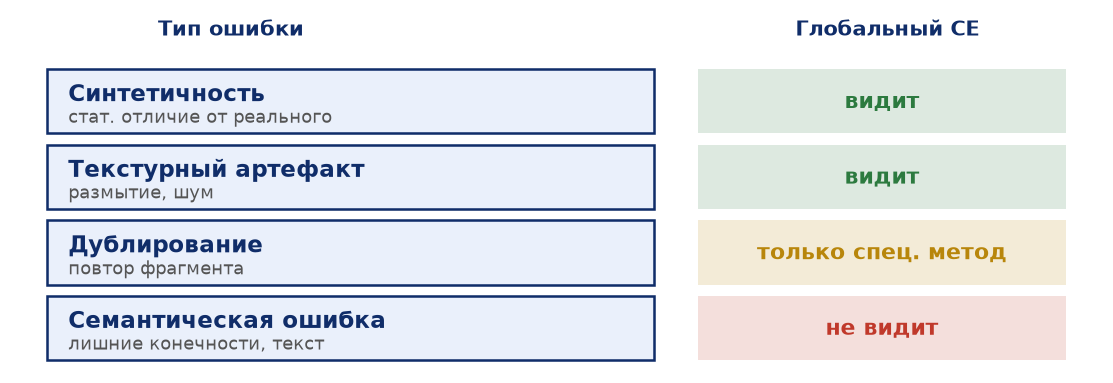
\includegraphics[width=\columnwidth]{fig_taxonomy}
\end{columns}
\end{frame}
\note{[СПИКЕР] Задача. Диффузионные модели порождают ошибки разной природы — от текстурных артефактов до семантических. Я изучаю, как параметры лёгкого дескриптора на основе сложности–энтропии влияют на оценку этих ошибок, и проверяю две гипотезы: H1 — отличить реальное от синтетического, H2 — отличить удачные генерации от неудачных. Справа — таксономия: чего от метода стоит ожидать.
[ПОЯСНЕНИЯ] CE — порядковая статистика яркостей (какой пиксель больше соседнего); по ней энтропия и сложность. Семантические галлюцинации не меняют локальную статистику, поэтому метод их видеть не обязан.}

% ========== МЕТОД ==========
\begin{frame}\frametitle{Метод}\framesubtitle{Лёгкий детерминированный конвейер + строгий протокол}
\begin{center}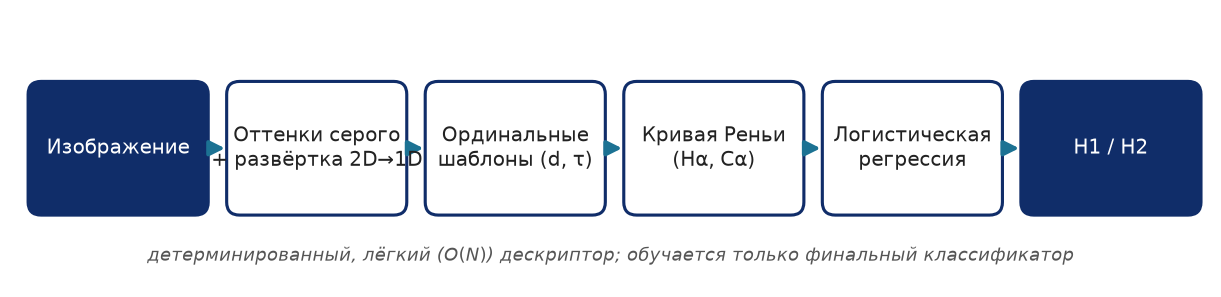
\includegraphics[width=0.96\textwidth]{fig_pipeline}\end{center}
\medskip
{\small Протокол: логистическая регрессия + повторная кросс-валидация + бутстреп-ДИ + тест ДеЛонга + контроль FDR. Исправлен дефект исходной (бакалаврской) работы — необучаемая случайная свёртка.}
\end{frame}
\note{[СПИКЕР] Метод. Изображение переводится в оттенки серого, разворачивается в сигнал, по нему строятся порядковые шаблоны и кривая Реньи; финальное решение даёт логистическая регрессия. Оценка — строгая: повторная кросс-валидация, доверительные интервалы, тест ДеЛонга, контроль ложных открытий. Работа продолжает мою бакалаврскую и исправляет её дефект — необучаемую случайную свёртку, дававшую шум.
[ПОЯСНЕНИЯ] Все шаги, кроме классификатора, детерминированы и линейны по числу пикселей — отсюда «лёгкий». AUROC: 0.5 — случайность, 1 — идеал.}

% ========== МЕТОД: дескриптор ==========
\begin{frame}\frametitle{Дескриптор и его инвариантность}
\begin{center}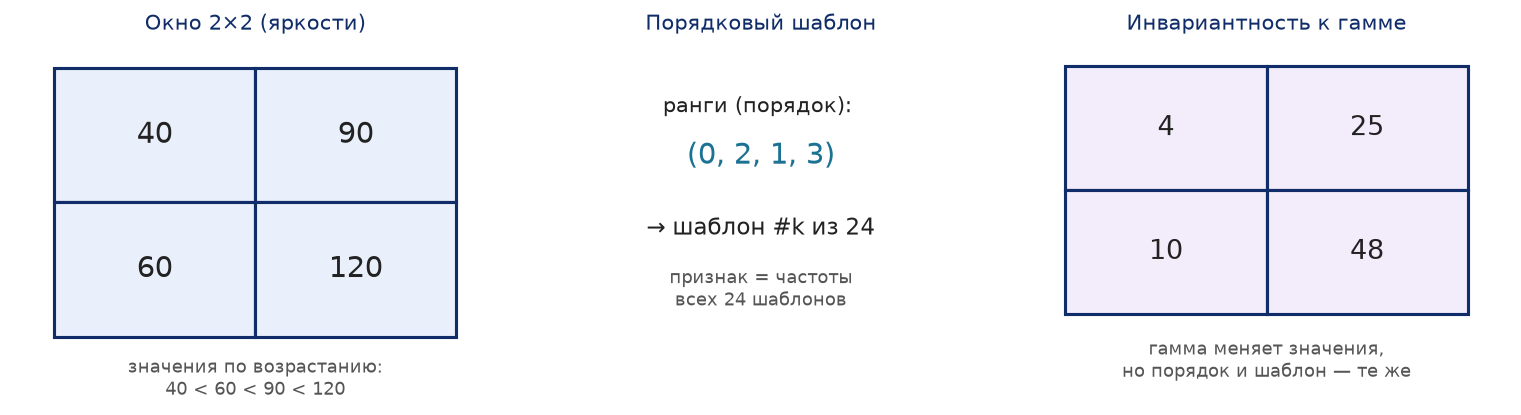
\includegraphics[width=0.95\textwidth]{fig_ordinal}\end{center}
\medskip
{\small Шаблон зависит только от \emph{порядка} яркостей $\Rightarrow$ инвариантность к монотонной тоновой правке (лемма~1). Это свойство далее даёт устойчивость прикладного метода.}
\end{frame}
\note{[СПИКЕР] Сам дескриптор: в окне два на два смотрим относительный порядок яркостей — это порядковый шаблон, один из 24; признак изображения — частоты всех шаблонов. Ключевое: шаблон зависит только от порядка, поэтому изменение яркости или гаммы его не меняет. Это лемма 1, и именно она даёт устойчивость прикладного детектора.
[ПОЯСНЕНИЯ] Справа та же область после гамма-коррекции: значения другие, порядок и шаблон те же. Этим ординальный подход отличается от методов на абсолютных интенсивностях.}

% ========== РЕЗУЛЬТАТЫ ==========
\begin{frame}\frametitle{Результаты}\framesubtitle{Сигнал есть для синтетичности, нет для галлюцинаций}
\begin{columns}
\column{0.38\textwidth}
\begin{exampleblock}{H1}\textbf{AUROC до 0{,}86}; CIFAKE 0{,}76.\end{exampleblock}
\begin{alertblock}{H2}\textbf{0 из 44} значимы (ДеЛонг + FDR).\end{alertblock}
\column{0.62\textwidth}
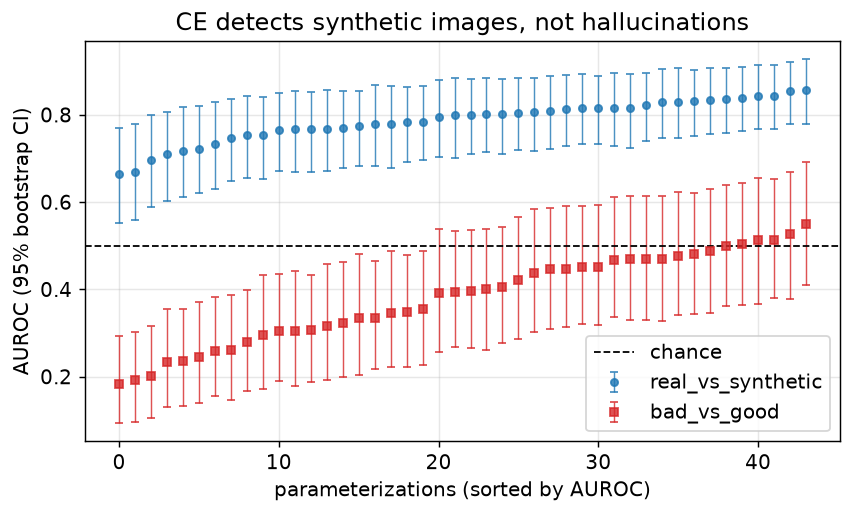
\includegraphics[width=\columnwidth]{fig_two_tasks}
\end{columns}
\medskip
{\footnotesize Честность: CE не превосходит спектр Фурье; часть H1 — конфаунд источника (метаданные дают 0{,}94), надёжен сбалансированный CIFAKE.}
\end{frame}
\note{[СПИКЕР] Результаты. По H1 сигнал есть: AUROC до 0.86 и 0.76 на независимом CIFAKE. По H2 сигнала нет: из 44 конфигураций ни одна не превышает случайность значимо. Важно честно: CE не лучше обычного спектра Фурье, а часть внутридоменного H1 — это конфаунд источника, поэтому надёжнее сбалансированный CIFAKE. Вывод: метод измеряет синтетичность, семантические галлюцинации недоступны.
[ПОЯСНЕНИЯ] H1 — реальное против синтетического; H2 — среди генераций удачные против неудачных. Конфаунд: метаданные файла (формат, разрешение, размер) сами разделяют классы с AUROC 0.94, то есть могли «подсказывать» ответ.}

% ========== РЕЗУЛЬТАТЫ: параметры ==========
\begin{frame}\frametitle{Результаты: влияние параметров}\framesubtitle{Качество управляется задержкой и схемой развёртки}
\begin{center}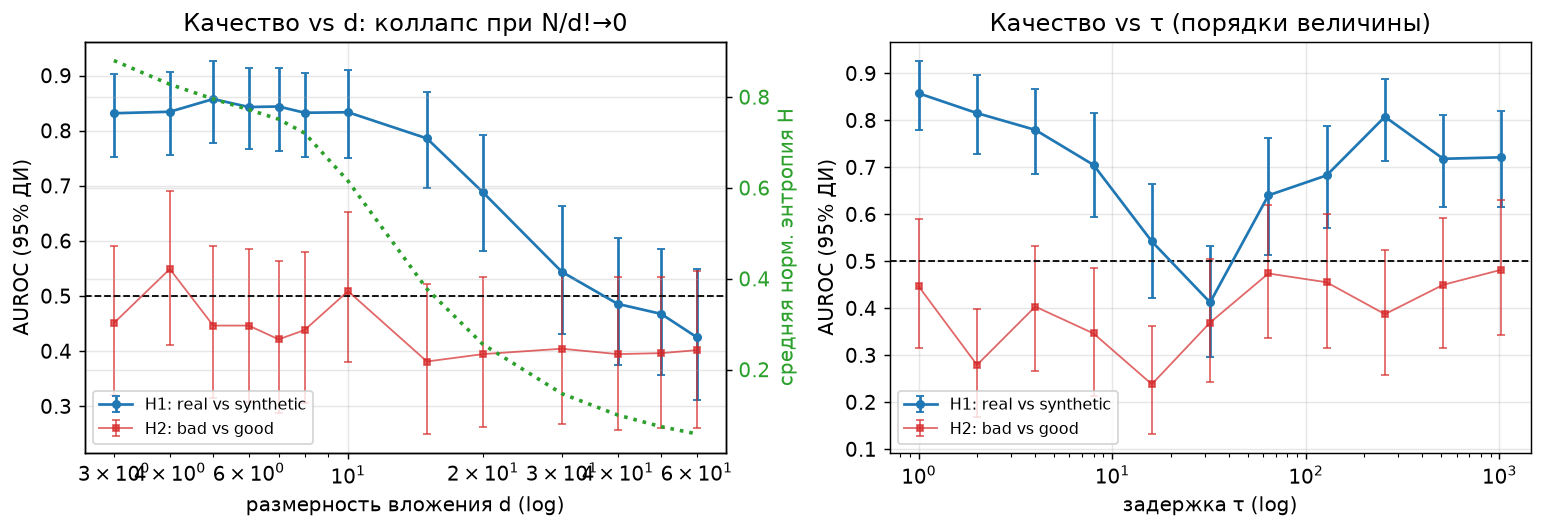
\includegraphics[width=0.96\textwidth]{fig_extended}\end{center}
\vspace{-1mm}
{\footnotesize $\tau=1$ лучше; растровые схемы $>$ кривой Гильберта; потолок размерности $d$ (статистика вырождается); резонанс при $\tau=$ ширине изображения.}
\end{frame}
\note{[СПИКЕР] Параметрический анализ — это ядро темы. Качество определяется задержкой и схемой развёртки: единичная задержка лучше, строчный растр обходит кривую Гильберта. По размерности — жёсткий потолок: число шаблонов растёт факториально, статистика вырождается. И отдельная находка — резонанс качества, когда задержка равна ширине изображения: развёртка тогда сэмплирует вертикальных соседей.
[ПОЯСНЕНИЯ] Для размерности d существует d! шаблонов; при d=10 это 3,6 млн — больше числа пикселей, поэтому оценка рассыпается. Резонанс связывает параметр с геометрией изображения.}

% ========== НОВИЗНА ==========
\begin{frame}\frametitle{Новизна: детектор дублирования}\framesubtitle{Применимый результат, устойчивый к тоновой маскировке}
\begin{center}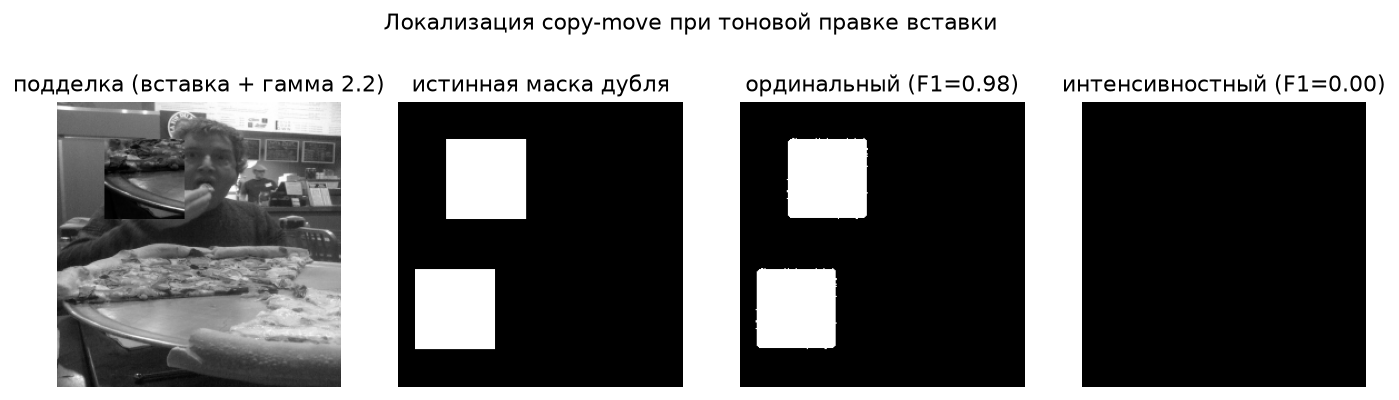
\includegraphics[width=0.82\textwidth]{fig_copymove_qual}\end{center}
\vspace{-1mm}
{\footnotesize Лёгкий детерминированный детектор-локализатор copy-move: \textbf{F1 0{,}93}, MCC 0{,}86. Устойчив к тоновой правке вставки (интенсивностный метод $\to$ случайность); инвариантен к отражению и повороту $90^\circ$.}
\end{frame}
\note{[СПИКЕР] Главная новизна. Из единственного положительного сигнала я довёл до конца прикладной метод — лёгкий детерминированный детектор-локализатор дублирования. С калиброванным порогом — F1 0.93, коэффициент Мэтьюса 0.86. Его преимущество выведено из доказанной инвариантности: он устойчив к подгонке яркости вставки, на которой интенсивностные методы падают к случайности; кольцевой вариант добавляет устойчивость к отражению и повороту на 90 градусов. На картинке: ординальный метод находит обе области, интенсивностный — ничего.
[ПОЯСНЕНИЯ] Copy-move — подделка, когда фрагмент копируется внутри изображения. F1 — баланс точности и полноты; MCC устойчив при дисбалансе. Порог калиброван без утечки (train/val по изображениям).}

% ========== ВЫВОДЫ ==========
\begin{frame}\frametitle{Выводы}
\begin{itemize}
	\item CE — дешёвый интерпретируемый дескриптор \textbf{синтетичности и локальных дефектов}; семантические галлюцинации он не решает;
	\item качество управляется задержкой и схемой развёртки (параметрический анализ);
	\item \textbf{новизна:} применимый детектор дублирования, устойчивый к тоновой и (частично) геометрической маскировке.
\end{itemize}
\begin{exampleblock}{Вклад}
\small Честный отрицательный результат с доказательствами + систематический параметрический анализ + доведённый до применимости лёгкий метод.
\end{exampleblock}
\end{frame}
\note{[СПИКЕР] Итог. Кривые сложности–энтропии — дешёвый интерпретируемый дескриптор синтетичности и локальных текстурных дефектов; задачу семантических галлюцинаций он не решает. Качество управляется прежде всего задержкой и схемой развёртки. Новизна — применимый детектор дублирования, устойчивый к тоновой и частично геометрической маскировке. Вклад работы: честный отрицательный результат с математическим объяснением, систематический параметрический анализ и доведённый до применимости лёгкий метод. Спасибо за внимание.
[ПОЯСНЕНИЯ] Для пятиминутного видео достаточно этих четырёх пунктов: задача, метод, результаты, новизна.}

\end{document}
